\documentclass{beamer}

% xcolor and define colors -------------------------
\usepackage{xcolor}

% https://www.viget.com/articles/color-contrast/
\definecolor{purple}{HTML}{5601A4}
\definecolor{navy}{HTML}{0D3D56}
\definecolor{ruby}{HTML}{9a2515}
\definecolor{alice}{HTML}{107895}
\definecolor{daisy}{HTML}{EBC944}
\definecolor{coral}{HTML}{F26D21}
\definecolor{kelly}{HTML}{829356}
\definecolor{cranberry}{HTML}{E64173}
\definecolor{jet}{HTML}{131516}
\definecolor{asher}{HTML}{555F61}
\definecolor{slate}{HTML}{314F4F}

% Mixtape Sessions
\definecolor{picton-blue}{HTML}{00b7ff}
\definecolor{violet-red}{HTML}{ff3881}
\definecolor{sun}{HTML}{ffaf18}
\definecolor{electric-violet}{HTML}{871EFF}

% Main theme colors
\definecolor{accent}{HTML}{00b7ff}
\definecolor{accent2}{HTML}{871EFF}
\definecolor{gray100}{HTML}{f3f4f6}
\definecolor{gray800}{HTML}{1F292D}


% Beamer Options -------------------------------------

% Background
\setbeamercolor{background canvas}{bg = white}

% Change text margins
\setbeamersize{text margin left = 15pt, text margin right = 15pt} 

% \alert
\setbeamercolor{alerted text}{fg = accent2}

% Frame title
\setbeamercolor{frametitle}{bg = white, fg = jet}
\setbeamercolor{framesubtitle}{bg = white, fg = accent}
\setbeamerfont{framesubtitle}{size = \small, shape = \itshape}

% Block
\setbeamercolor{block title}{fg = white, bg = accent2}
\setbeamercolor{block body}{fg = gray800, bg = gray100}

% Title page
\setbeamercolor{title}{fg = gray800}
\setbeamercolor{subtitle}{fg = accent}

%% Custom \maketitle and \titlepage
\setbeamertemplate{title page}
{
    %\begin{centering}
        \vspace{20mm}
        {\Large \usebeamerfont{title}\usebeamercolor[fg]{title}\inserttitle}\\
        {\large \itshape \usebeamerfont{subtitle}\usebeamercolor[fg]{subtitle}\insertsubtitle}\\ \vspace{10mm}
        {\insertauthor}\\
        {\color{asher}\small{\insertdate}}\\
    %\end{centering}
}

% Table of Contents
\setbeamercolor{section in toc}{fg = accent!70!jet}
\setbeamercolor{subsection in toc}{fg = jet}

% Button 
\setbeamercolor{button}{bg = accent}

% Remove navigation symbols
\setbeamertemplate{navigation symbols}{}

% Table and Figure captions
\setbeamercolor{caption}{fg=jet!70!white}
\setbeamercolor{caption name}{fg=jet}
\setbeamerfont{caption name}{shape = \itshape}

% Bullet points

%% Fix left-margins
\settowidth{\leftmargini}{\usebeamertemplate{itemize item}}
\addtolength{\leftmargini}{\labelsep}

%% enumerate item color
\setbeamercolor{enumerate item}{fg = accent}
\setbeamerfont{enumerate item}{size = \small}
\setbeamertemplate{enumerate item}{\insertenumlabel.}

%% itemize
\setbeamercolor{itemize item}{fg = accent!70!white}
\setbeamerfont{itemize item}{size = \small}
\setbeamertemplate{itemize item}[circle]

%% right arrow for subitems
\setbeamercolor{itemize subitem}{fg = accent!60!white}
\setbeamerfont{itemize subitem}{size = \small}
\setbeamertemplate{itemize subitem}{$\rightarrow$}

\setbeamertemplate{itemize subsubitem}[square]
\setbeamercolor{itemize subsubitem}{fg = jet}
\setbeamerfont{itemize subsubitem}{size = \small}







% Links ----------------------------------------------

\usepackage{hyperref}
\hypersetup{
  colorlinks = true,
  linkcolor = accent2,
  filecolor = accent2,
  urlcolor = accent2,
  citecolor = accent2,
}


% Line spacing --------------------------------------
\usepackage{setspace}
\setstretch{1.1}


% \begin{columns} -----------------------------------
\usepackage{multicol}


% Fonts ---------------------------------------------
% Beamer Option to use custom fonts
\usefonttheme{professionalfonts}

% \usepackage[utopia, smallerops, varg]{newtxmath}
% \usepackage{utopia}
\usepackage[sfdefault,light]{roboto}

% Small adjustments to text kerning
\usepackage{microtype}



% Remove annoying over-full box warnings -----------
\vfuzz2pt 
\hfuzz2pt


% Table of Contents with Sections
\setbeamerfont{myTOC}{series=\bfseries, size=\Large}
\AtBeginSection[]{
        \frame{
            \frametitle{Roadmap}
            \tableofcontents[current]   
        }
    }


% Tables -------------------------------------------
% Tables too big
% \begin{adjustbox}{width = 1.2\textwidth, center}
\usepackage{adjustbox}
\usepackage{array}
\usepackage{threeparttable, booktabs, adjustbox}
    
% Fix \input with tables
% \input fails when \\ is at end of external .tex file
\makeatletter
\let\input\@@input
\makeatother

% Tables too narrow
% \begin{tabularx}{\linewidth}{cols}
% col-types: X - center, L - left, R -right
% Relative scale: >{\hsize=.8\hsize}X/L/R
\usepackage{tabularx}
\newcolumntype{L}{>{\raggedright\arraybackslash}X}
\newcolumntype{R}{>{\raggedleft\arraybackslash}X}
\newcolumntype{C}{>{\centering\arraybackslash}X}

% Figures

% \imageframe{img_name} -----------------------------
% from https://github.com/mattjetwell/cousteau
\newcommand{\imageframe}[1]{%
    \begin{frame}[plain]
        \begin{tikzpicture}[remember picture, overlay]
            \node[at = (current page.center), xshift = 0cm] (cover) {%
                \includegraphics[keepaspectratio, width=\paperwidth, height=\paperheight]{#1}
            };
        \end{tikzpicture}
    \end{frame}%
}

% subfigures
\usepackage{subfigure}


% Highlight slide -----------------------------------
% \begin{transitionframe} Text \end{transitionframe}
% from paulgp's beamer tips
\newenvironment{transitionframe}{
    \setbeamercolor{background canvas}{bg=accent!40!black}
    \begin{frame}\color{accent!10!white}\LARGE\centering
}{
    \end{frame}
}


% Table Highlighting --------------------------------
% Create top-left and bottom-right markets in tabular cells with a unique matching id and these commands will outline those cells
\usepackage[beamer,customcolors]{hf-tikz}
\usetikzlibrary{calc}
\usetikzlibrary{fit,shapes.misc}

% To set the hypothesis highlighting boxes red.
\newcommand\marktopleft[1]{%
    \tikz[overlay,remember picture] 
        \node (marker-#1-a) at (0,1.5ex) {};%
}
\newcommand\markbottomright[1]{%
    \tikz[overlay,remember picture] 
        \node (marker-#1-b) at (0,0) {};%
    \tikz[accent!80!jet, ultra thick, overlay, remember picture, inner sep=4pt]
        \node[draw, rectangle, fit=(marker-#1-a.center) (marker-#1-b.center)] {};%
}

\usepackage{breqn} % Breaks lines

\usepackage{amsmath}
\usepackage{mathtools}

\usepackage{pdfpages} % \includepdf

\usepackage{listings} % R code
\usepackage{verbatim} % verbatim

% Video stuff
\usepackage{media9}

% packages for bibs and cites
\usepackage{natbib}
\usepackage{har2nat}
\newcommand{\possessivecite}[1]{\citeauthor{#1}'s \citeyearpar{#1}}
\usepackage{breakcites}
\usepackage{alltt}

% Setup math operators
\DeclareMathOperator{\E}{E} \DeclareMathOperator{\tr}{tr} \DeclareMathOperator{\se}{se} \DeclareMathOperator{\I}{I} \DeclareMathOperator{\sign}{sign} \DeclareMathOperator{\supp}{supp} \DeclareMathOperator{\plim}{plim}
\DeclareMathOperator*{\dlim}{\mathnormal{d}\mkern2mu-lim}
\newcommand\independent{\protect\mathpalette{\protect\independenT}{\perp}}
   \def\independenT#1#2{\mathrel{\rlap{$#1#2$}\mkern2mu{#1#2}}}
\newcommand*\colvec[1]{\begin{pmatrix}#1\end{pmatrix}}

\newcommand{\myurlshort}[2]{\href{#1}{\textcolor{gray}{\textsf{#2}}}}


\begin{document}

\imageframe{./lecture_includes/mixtape_did_cover.png}


% ---- Content ----


\section{Basic DiD}

\subsection{Simple case, no covariates}

\begin{frame}{Introducing DiD}

\begin{itemize}
\item DiD in its modern form dates back to Orley Ashenfelter and David Card at Princeton in the late 70s and mid 80s (Card says they invent the term in mid 1980s)
\item Unclear when key identifying assumptions like parallel trends are worked out (as originally there is no potential outcomes in play)
\item Attractive elements included natural experimentation, panel data, and did not require randomization
\item US context may also have been such that it had a lot of upside
\item But let's start at the beginning with story and example
\end{itemize}

\end{frame}

\begin{frame}{Miasma Debates}

\begin{itemize}

\item Health policy debates in the 19th century is where we DiD pop up, mainly as a matter of logical deduction 
\item Dominant disease theory in 19th century was \emph{miasma} -- disease caused by smelly vapor
\item Helped fuel a lot of sanitation reforms, but inadequate for explaining many diseases 
\item ``All models are wrong but some are useful'' -- George Box)
\item Keep in mind -- microorganisms would not be identified until much later, partly caused by poor resolution in microscopes (Freedman 2007)

\end{itemize}

\end{frame}

\begin{frame}{Miasma I: Ignaz Semmelweis}

\begin{itemize}
\item 1840s, Vienna maternity wards had high postpartum infections in one wing compared to other wings
\item One division had doctors and trainee doctors, but another had midwives and trainee midwives
\item Ignaz Semmelweis notes the difference in 1841 when hospitals moved to ``anatomical'' training involving cadavers (Jakeila lecture 4, DiD)
\item New training happens to one but not the other and Semmelweis thinks the mortality is caused by working with cadavers
\item Proposes washing hands with chlorine in 1847 in the midwives' wing and uses a DiD design of pre and post
\end{itemize}

\end{frame}



\begin{frame}{Miasma II: John Snow and cholera}

\begin{itemize}
\item More well known involves John Snow, an important inventor of a device that delivered chloroform to patients for surgery (major advancement in anesthesia)
\item H was also an amateur epidemiologist in 19th century, and these days it's more common to hear him be named the father of DiD
\item Believed cholera was spread through the Thames water supply which contradicted dominant theory about ``dirty air'' transmission
\item Grand experiment: Lambeth moves its pipe between 1849 and 1854; Southwark and Vauxhall delay
\item How can he use this event to test his hypothesis? Three ways: simple comparisons, interrupted time series of the difference in differences (DiD)
\end{itemize}

\end{frame}





\begin{frame}{Simple cross-sectional design}

\begin{table}\centering
		\caption{Lambeth and Southwark and Vauxhall, 1854}
		\begin{center}
		\begin{tabular}{ll}
		\toprule
		\multicolumn{1}{l}{\textbf{Company}}&
		\multicolumn{1}{c}{\textbf{Cholera mortality}}\\
		\midrule
		Lambeth  & $Y=L + D$ \\
		\midrule
		Southwark and Vauxhall  & $Y=SV$ \\
		\bottomrule
		\end{tabular}
		\end{center}
	\end{table}

\bigskip

\begin{eqnarray*}
\widehat{\delta}_{cs} = D + (L-SV)
\end{eqnarray*}This is selection bias with respect to $Y^0$.

\end{frame}

\begin{frame}{Interrupted time series design}

	\begin{table}\centering
		\caption{Lambeth, 1849 and 1854}
		\begin{center}
		\begin{tabular}{lll}
		\toprule
		\multicolumn{1}{l}{\textbf{Company}}&
		\multicolumn{1}{c}{\textbf{Time}}&
		\multicolumn{1}{c}{\textbf{Cholera mortality}}\\
		\midrule
		Lambeth & 1849 & $Y=L$ \\
		& 1854 & $Y=L + (T + D)$ \\
		\bottomrule
		\end{tabular}
		\end{center}
	\end{table}

\begin{eqnarray*}
\widehat{\delta}_{its} = D + T
\end{eqnarray*}This is selection bias with respect to time, $T \neq 0$


\end{frame}

\begin{frame}{Difference-in-differences}

\begin{table}\centering
		\caption{Lambeth and Southwark and Vauxhall, 1849 and 1854}
		\begin{center}
		\begin{tabular}{lll|lc}
		\toprule
		\multicolumn{1}{l}{\textbf{Companies}}&
		\multicolumn{1}{c}{\textbf{Time}}&
		\multicolumn{1}{c}{\textbf{Outcome}}&
		\multicolumn{1}{c}{$D_1$}&
		\multicolumn{1}{c}{$D_2$}\\
		\midrule
		Lambeth & Before & $Y=L$ \\
		& After & $Y=L + T_L + D$ & $T_L+D$\\
		\midrule
		& & & & $D$ \\
		\midrule
		Southwark and Vauxhall & Before & $Y=SV$ \\
		& After & $Y=SV + T_{SV}$ & $T_{SV}$\\
		\bottomrule
		\end{tabular}
		\end{center}
	\end{table}

\begin{eqnarray*}
\widehat{\delta}_{did} = D + (T_L - T_{SV})
\end{eqnarray*}This is selection bias with respect to $Y^0$ trends

\end{frame}

\begin{frame}{DiD equation, 2x2 and parallel trends}

\begin{itemize}
\item I tend to group DiD based on whether the design will be based on two things:
	\begin{enumerate}
	\item \textbf{Parallel trends}: $T_L = T_{SV}$ for identification
	\item \textbf{DiD equation}: (After minus before for treated) - (After minus before for comparison group)
	\end{enumerate}
\item Goodman-Bacon (2018; 2021) calls the DiD equation the ``2x2'' and I will too sometimes, but they mean the same thing
\item Both tend to show up repeatedly in each of the methods we examine in this workshop
\item It's how I differentiate DiD from others like the broadly defined panel estimators
\end{itemize}

\end{frame}






\begin{frame}{DiD equation with sample averages}

\begin{eqnarray*}
\widehat{\delta}^{2x2}_{kU} = \bigg ( \overline{y}_k^{post(k)} - \overline{y}_k^{pre(k)} \bigg ) - \bigg ( \overline{y}_U^{post(k)} - \overline{y}_U^{pre(k)} \bigg )
\end{eqnarray*}

\end{frame}

\begin{frame}{DiD equation with population expectations}

\begin{eqnarray*}
\widehat{\delta}^{2x2}_{kU} = \bigg ( E[Y_k|Post] - E[Y_k|Pre] \bigg ) - \bigg ( E[Y_U | Post ] - E[ Y_U | Pre] \bigg) \\
\end{eqnarray*}

\end{frame}


\begin{frame}{Potential outcomes and the switching equation}

\begin{eqnarray*}
\widehat{\delta}^{2x2}_{kU} &=& \bigg ( \underbrace{E[Y^1_k|Post] - E[Y^0_k|Pre] \bigg ) - \bigg ( E[Y^0_U | Post ] - E[ Y^0_U | Pre]}_{\mathclap{\text{Switching equation}}} \bigg)  \\
&&+ \underbrace{\textcolor{red}{E[Y_k^0 |Post] - E[Y^0_k | Post]}}_{\mathclap{\text{Adding zero}}} 
\end{eqnarray*}

\end{frame}

\begin{frame}{Parallel trends bias}

\begin{eqnarray*}
\widehat{\delta}^{2x2}_{kU} &=& \underbrace{E[Y^1_k | Post] - \textcolor{red}{E[Y^0_k | Post]}}_{\mathclap{\text{ATT}}} \\
&& + \bigg [  \underbrace{\textcolor{red}{E[Y^0_k | Post]} - E[Y^0_k | Pre] \bigg ] - \bigg [ E[Y^0_U | Post] - E[Y_U^0 | Pre] }_{\mathclap{\text{Non-parallel trends bias in 2x2 case}}} \bigg ]
\end{eqnarray*}

\bigskip

Note that this is what we saw in the table earlier -- $T_L \neq T_{SV}$ and it's not measurable because $T_L$ is confounded by the ATT itself


\end{frame}

\begin{frame}{Similar role $Y^0$ in selection bias}

Cross-sectional comparisons and selection bias with respect to $Y^0$

\begin{eqnarray*}
E[Y|D=1] - E[Y|D=0] &=& ATE + E[Y^0|D=1] - E[Y^0|D=0] \\
&=& + (1- \pi)(ATT-ATU)
\end{eqnarray*}

DiD comparisons and selection bias with respect to $Y^0$

\begin{eqnarray*}
\widehat{\delta}^{2x2}_{kU} &=& \underbrace{E[Y^1_k | Post] - \textcolor{red}{E[Y^0_k | Post]}}_{\mathclap{\text{ATT}}} \\
&& + \bigg [  \underbrace{\textcolor{red}{E[Y^0_k | Post]} - E[Y^0_k | Pre] \bigg ] - \bigg [ E[Y^0_U | Post] - E[Y_U^0 | Pre] }_{\mathclap{\text{Non-parallel trends bias in 2x2 case}}} \bigg ]
\end{eqnarray*}

\end{frame}


\begin{frame}{Independence}
	

	\begin{block}{Independence assumption}
	Treatment is assigned to a population independent of that population's potential outcomes  $$(Y^0,Y^1)\independent{D}$$
	\end{block}
This is random or quasi-random assignment and ensures mean potential outcomes for the treatment group and control group are the same.  Also ensures other variables are distributed the same for a large sample.
		\begin{eqnarray*}
			E[Y^0|D=1] &=& E[Y^0 | D=0] \\
			E[Y^1|D=1] &=& E[Y^1 | D=0] 
		\end{eqnarray*}
\end{frame}

\begin{frame}{Non-randomization identification}

\begin{itemize}
\item But we won't use randomization for identification with DiD
\item This is one of the appeals of DiD -- we aren't using physical randomization
\item But note, independence works and gives confidence ``because we know how the science works'' -- Don Rubin
\item There is no such ``science'' with parallel trends, so we tend to focus on a variety of ad hoc tests like event studies for confidence
\item But otherwise, it's actually quite similar, and shows that identification does not always depend on randomization
\end{itemize}

\end{frame}


\begin{frame}{OLS Specification}
	
	\begin{itemize}
	\item Simple difference in means can be computed with OLS, too, but not as easy to explicitly see the parallel trends so I'll show you graphically
	\item Properly specified OLS model will also identify the ATT when there is only two groups and no covariates
	\item Often preferred because
		\begin{itemize}
		\item OLS estimates the ATT under parallel trends
		\item Easy to calculate the standard errors
		\item Easy to include multiple periods
		\end{itemize}
	\item But some issues emerge with differential timing, time varying covariates and continuous treatments
	\end{itemize}
\end{frame}

\begin{frame}{Minimum wages}

\begin{itemize}
\item Card and Krueger (1994) have a famous study estimating causal effect (ATT) of minimum wages on employment
\item Exploited a policy change in New Jersey between February and November in mid-1990s where minimum wage was increased
\item Neighbor PA did not (remember no spillover assumption)
\item Found no effect on minimum wage; if anything it was the opposite effect
\item Caused some feuding with Buchanan saying people who believed it enough to adopt it were ``camp following whores'' (Wall Street Journal op-ed during Clinton admin)
\end{itemize}

\end{frame}

\begin{frame}{OLS specification of the DiD equation}
	
	\begin{itemize}
	\item The equivalent regression includes time and group fixed effects:$$Y_{its} = \alpha + \gamma NJ_s + \lambda d_t + \delta (NJ \times d)_{st} + \varepsilon_{its}$$
		\begin{itemize}
		\item NJ is a dummy equal to 1 if the observation is from NJ
		\item d is a dummy equal to 1 if the observation is from November (the post period)
		\end{itemize}
	\item This equation takes the following values
		\begin{itemize}
		\item PA Pre: $\alpha$
		\item PA Post: $\alpha + \lambda$
		\item NJ Pre: $\alpha + \gamma$
		\item NJ Post: $\alpha + \gamma + \lambda + \delta$
		\end{itemize}
	\item DiD equation: (NJ Post - NJ Pre) - (PA Post - PA Pre) $= \delta$
	\end{itemize}
\end{frame}




\begin{frame}[plain]
	$$Y_{ist} = \alpha + \gamma NJ_s + \lambda d_t + \delta(NJ\times d)_{st} + \varepsilon_{ist}$$
	\begin{figure}
	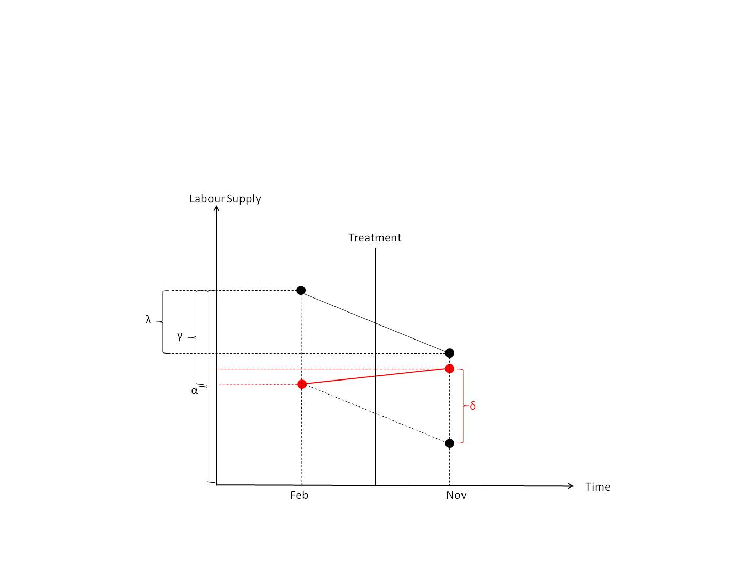
\includegraphics[scale=0.90]{./lecture_includes/waldinger_dd_5.pdf}
	\end{figure}
\end{frame}

\begin{frame}{OLS with twoway fixed effects}


Under parallel trends, OLS estimates the ATT. Researchers often will use OLS with time-varying covariates, but this is not advised as it is only unbiased under more restrictive assumptions which we discuss next (though see new working paper by Cattaneo, et al. 2022 on controlling for time-varying covariates).



\end{frame}


\subsection{IPW}




\begin{frame}{Inverse probability weighting DiD}

\begin{itemize}
\item Abadie (2005) proposed a DiD estimator that could incorporate covariates and get an unbiased estimate of the ATT
\item Researcher needs treatment and comparison group observed before and after treatment
\item If treatment group units are selected based on their (observed) covariates, then baseline covariates are also needed 
\end{itemize}

\end{frame}


\begin{frame}{Time varying versus time invariant covariates}

\begin{itemize}
\item In a DiD, we may need to control for X because treatment is only conditional on X
\item But in TWFE, all time invariant covariates are absorbed by the unit fixed effects -- only time varying covariates will survive TWFE
\item But time varying covariates place restrictions, as we will see, on the DGP and run the threat of conditioning on outcomes if they were changed by the treatment
\item Abadie proposes using only the covariates at baseline to form weights in the simple DiD formula
\end{itemize}

\end{frame}

\begin{frame}{Three step method}

\begin{enumerate}
\item Compute each unit's ``after minus before'' which is the DD part
\item Then estimate a propensity score which you'll use to weight each unit
\item Finally, compare weighted changes in ``after minus before'' for treatment versus comparison groups
\end{enumerate}

\bigskip

You can have heterogeneous treatment effects, but not differential timing

\end{frame}

\begin{frame}{Terms}

\begin{itemize}
\item $t$ is year of treatment which doesn't vary across units (so no differential timing)
\item $Y^1$ and $Y^0$ are potential outcomes (counterfactual versus actual)
\item $D$ is 1 or 0 based on group and time
\item $b$ is the ``baseline'' which is similar to CS using $g$ as the one year pre-treatment
\item $X$ are ``baseline'' covariates \textbf{only} -- they do not vary over time, which means propensity scores are estimated off the $b$ period \textbf{only}
\end{itemize}

\end{frame}

\begin{frame}{Assumptions}

Kind of common for this propensity score literature to only have two assumptions.  But usually the first conditional independence.  Now it is parallel trends because this is DD

\begin{enumerate}
\item Conditional parallel trends $$E[Y^0_t - Y^0_b|D=1,X_b] - E[Y^0_t - Y^0_t | D=0, X_b]$$ (Notice the $b$ subscript.  What is that you think?)
\item Common support $$Pr(D=1)>0; Pr(D=1|X)<1$$ Let's see a picture of common support that I drew.  Apologies it's horrible
\end{enumerate}

\end{frame}

\begin{frame}{Common support}

As we are identifying the ATT, we only need common support with respect to treated units

\bigskip

Your identify assumptions are always with respect to the missing covariates in other words and for the ATT, you are missing $Y^0$ for the treatment group

\bigskip

If we were estimating ATU, we'd be missing $Y^1$ for controls and need common support ($Y$ in treatment for all ranges of control), and for ATE we'd need both

\end{frame}

\begin{frame}{Visualizing propensity score to get common support}

	\begin{figure}
	\includegraphics[scale=0.05]{./lecture_includes/common_support_abadie.png}
	\end{figure}

\end{frame}

\begin{frame}{Definition and estimation}

Defining the ATT parameter of interest
\begin{equation}
ATT=E[Y^1_t - Y^0_t |D_t=1]
\end{equation}

\bigskip
Abadie's estimator
\begin{equation}
E\bigg [ \frac{Y_t - Y_b}{Pr(D_t=1)} \times \frac{D_t - Pr(D=1|X_b)}{1-Pr(D=1|X_b)} \bigg ]
\end{equation}


\end{frame}


\begin{frame}{Propensity scores}

\begin{itemize}
\item Paper is titlted ``Semi-parametric DiD'' because Abadie imposes structure on the polynomials used to construct the propensity score
\item You can use OLS linear probability models or series logit estimation
\end{itemize}

\end{frame}

\begin{frame}{Estimating propensity scores}

It's common to hear people say that we don't know the propensity score; we can only estimate it. Same here -- we approximate it with regressions

\bigskip

\begin{equation}
\widehat{Pr}(X_b) = \widehat{\gamma_0} + \widehat{\gamma_1}X + \widehat{\gamma_2}X^2 + \dots \varepsilon
\end{equation}

\bigskip

\begin{equation}
\widehat{Pr}(X_b) =  F(\widehat{\gamma_0} + \widehat{\gamma_1}X + \widehat{\gamma_2}X^2 + \dots)
\end{equation}

\end{frame}


\begin{frame}{Commentary on paper's influence}

Abadie has a great year in 2003: synthetic control in AER, semiparametric DiD in Restud, semiparametric IV (his JMP) in JoE

\bigskip

Semiparametric DiD has over 2,000 cites

\bigskip

But I'm not sure it was widely adopted by the \emph{applied} community. It seems like the \emph{applied community} starts paying attention to the econometric contributions much later, and Abadie (2003) is gaining a renaissance at the moment because of the next paper

\bigskip

Nonetheless, there is code in Stata called -absdid- but an unsatisfying part of the semiparametric piece is that the results change with respect to not just the estimation method (OLS or logit), but also with respect to the order in which the covariates appear

\end{frame}



\subsection{DRDiD}

\begin{frame}{Doubly Robust Difference-in-differences}

\begin{itemize}
\item DR models control for covariates twice -- once using the propensity score, once using outcomes adjusted by regression -- and are unbiased so long as:
	\begin{itemize}
	\item The regression specification for the outcome is correctly specified
	\item The propensity score specification is correctly specified
	\end{itemize}
\item Sant'Anna and Zhao (2020) incorporated DR into DiD by combining inverse probability weighting and outcome regression into a single DiD model
\item It's in the engine of Callaway and Sant'Anna (2020) that we discuss later so it merits close study
\item One of my favorite lesser known of the new DiD papers
\end{itemize}

\end{frame}

\begin{frame}{Patterns in econometrician reasoning}

\begin{enumerate}
\item Define the target parameter first (as opposed to writing down model first)
\item Identification (e.g., parallel trends)
\item Estimation
\item Aggregation
\item Inference
\end{enumerate}

\end{frame}


\begin{frame}{Defining the target parameter}

Major part of the new econometrics is to always start with the target parameter and build to it using estimation and identification that ``works''

\bigskip

\begin{eqnarray*}
\delta = E[Y^1_{it} - Y^0_{it} | D_i=1]
\end{eqnarray*}

\end{frame}

\begin{frame}{Identification assumptions I: Data}

Assumption 1: Assume panel data or repeated cross-sectional data

\bigskip

Handling repeated cross-sectional data is possible but assumes modularity which is a kind of stability assumption, but I'll use panel representation. 

\bigskip

Cross-sections will be potentially violated with changing sample compositions (see my Mixtape on the Napster example). 

\end{frame}

\begin{frame}{Identification assumptions II: Modification to parallel trends}

Assumption 2: Conditional parallel trends

\bigskip

Counterfactual trends for the treatment group are the same as the control group for all values of $X$

\begin{eqnarray*}
E[Y_1^0 - Y_0^0 | X, D=1] = E[Y^0_1 - Y^0_0 | X, D=0]
\end{eqnarray*}

\end{frame}

\begin{frame}{Identification assumptions III: Common support}

Assumption 3: Common support

\bigskip

For some $e>0$, the probability of being in the treatment group is greater than $e$ and the probability of being in the treatment group conditional on $X$ is $\leq1-e$. 

\bigskip

Intuition of assumption 3: Called overlap or common support. Means there is at least a small fraction of the population that is treated and that for every value of the covariates $X$ there is at least a small chance that the unit is not treated. It's called common support when it's a propensity score but it's just about the distribution of treatment and control across values of $X$. Very common when dealing with covariate comparisons as otherwise you're extrapolating (curse of dimensionality)

\end{frame}

\begin{frame}{Estimating DD with Assumptions 1-3}

\begin{itemize}
\item Assumptions 1-3 gives us a couple of options of estimating the DiD
\item We can either use the outcome regression (OR) approach of Heckman, et al 1997
\item Or we can use the inverse probability weighting (IPW) approach of Abadie (2005)
\end{itemize}

\end{frame}


\begin{frame}{Outcome regression}

This is the Heckman, et al. (1997) approach where the outcome evolution is modeled with a regression

\bigskip

\begin{eqnarray*}
\widehat{\delta}^{OR} = \overline{Y}_{1,1} - \bigg [ \overline{Y}_{1,0} + \frac{1}{n^T} \sum_{i|D_i=1} ( \widehat{\mu}_{0,1}(X_i) - \widehat{\mu}_{0,0}(X_i)) \bigg ]
\end{eqnarray*}

where $\overline{Y}$ is the sample average of $Y$ among units in the treatment group at time $t$ and $\widehat{\mu}(X)$ is an estimator of the true, but unknown, $m_{d,t}(X)$ which is by definition equal to $E[Y_t|D=d,X=x]$.

\end{frame}




\begin{frame}{Outcome regression}

\begin{eqnarray*}
\widehat{\delta}^{OR} = \overline{Y}_{1,1} - \bigg [ \overline{Y}_{1,0} + \frac{1}{n^T} \sum_{i|D_i=1} ( \widehat{\mu}_{0,1}(X_i) - \widehat{\mu}_{0,0}(X_i)) \bigg ]
\end{eqnarray*}

\begin{enumerate}
\item Regress changes $\Delta Y$ on $X$ among untreated groups using baseline covariates only
\item Get fitted values of the regression using all $X$ from $D=1$ only.  Average those
\item Calculate change in this fitted $Y$ among treated with the average fitted values
\end{enumerate}

\end{frame}

\begin{frame}{Inverse probability weighting}

This is the Abadie (2005) approach where we use weighting

\begin{eqnarray*}
\widehat{\delta}^{ipw} = \frac{1}{E_N[D]} E \bigg [ \frac{D-\widehat{p}(X)}{1-\widehat{p}(X)} (Y_1-Y_0) \bigg ]
\end{eqnarray*}

where $\widehat{p}(X)$ is an estimator for the true propensity score. Reduces the dimensionality of $X$ into a single scalar.

\end{frame}

\begin{frame}{These models cannot be ranked}

\begin{itemize}
\item Outcome regression needs $\widehat{\mu}(X)$ to be correctly specified, whereas
\item Inverse probability weighting needs $\widehat{p}(X)$ to be correctly specified
\item It's hard to ``rank'' these two in practice with regards to model misspecification because each is inconsistent when their own models are misspecified
\item Well why don't we just use TWFE?  I've never heard anyone complain about including covariates in TWFE and I've been doing it my entire adult life, so we're good right?
\item Depends on if you want to assume three more things. 
\end{itemize}

\end{frame}

\begin{frame}{TWFE}

Here's the TWFE specification:

\begin{eqnarray*}
Y_{it} = \alpha_1  + \alpha_2 T_t + \alpha_3 D_i +  \delta (T_i \times D_t)  + \varepsilon_{it}
\end{eqnarray*}

\bigskip

Just add in covariates then right?

\begin{eqnarray*}
Y_{it} = \alpha_1  + \alpha_2 T_t + \alpha_3 D_i  + \delta (T_i \times D_t) + \theta \cdot X_{it} + \varepsilon_{it}
\end{eqnarray*}

Sure! If you're willing to impose three \emph{more} assumptions

\end{frame}




\begin{frame}{Decomposing TWFE with covariates}

TWFE places restrictions on the DGP. Previous TWFE regression under assumptions 1-3 implies the following:

\bigskip

\begin{eqnarray*}
E[Y^1_1|D=1,X] = \alpha_1 + \alpha_2 + \alpha_3 + \delta + \theta X
\end{eqnarray*}

\bigskip

Conditional parallel trends implies

\small
\begin{eqnarray*}
&&E[Y^0_{1} - Y^0_{0}|D=1,X]= E[Y^0_{1} - Y^0_{0}|D=0,X] \\
&&E[Y^0_{1}|D=1,X] - E[Y^0_{0}|D=1,X]= E[Y^0_{1}|D=0,X] - E[Y^0_{0}|D=0,X] \\
&&E[Y^0_{1}|D=1,X] = E[Y^0_{0}|D=1,X] + E[Y^0_{1}|D=0,X] - E[Y^0_{0}|D=0,X] \\
&&E[Y^0_{1}|D=1,X] = E[Y_{0}|D=1,X] + E[Y_{1}|D=0,X] - E[Y_{0}|D=0,X] \\
\end{eqnarray*}


\end{frame}

\begin{frame}{Switching equation substitution}

Last line from the switching equation. This gives us:

\begin{eqnarray*}
E[Y^0_{1}|D=1,X] = \alpha_1  + \alpha_2 + \alpha_3 + \theta X
\end{eqnarray*}

Now compare this with our earlier $Y^1$ expression

\begin{eqnarray*}
E[Y^1_1|D=1,X] = \alpha_1 + \alpha_2 + \alpha_3 + \delta + \theta X
\end{eqnarray*}

We can define our target parameter, the ATT, now in terms of the fixed effects representation

\end{frame}


\begin{frame}{Collecting terms}

TWFE representation of our conditional expectations of the potential outcomes
\begin{eqnarray*}
&&E[Y^1_1|D=1,X] = \alpha_1 + \alpha_2 + \alpha_3 + \delta + \theta_1 X \\
&&E[Y^0_{1}|D=1,X] = \alpha_1  + \alpha_2 + \alpha_3 + \theta_2 X \\
\end{eqnarray*}

Substitute these into our target parameter

\begin{eqnarray*}
ATT &=& E[Y^1_1|D=1,X]  - E[Y^0_{1}|D=1,X]   \\
&&=(\alpha_1 + \alpha_2 + \alpha_3 + \delta + \theta_1 X) - ( \alpha_1  + \alpha_2 + \alpha_3 + \theta_2 X )\\
&&=\delta + (\theta_1 X - \theta_2 X)
\end{eqnarray*}

\bigskip

What if $\theta_1 X \neq \theta_2 X$?

\end{frame}

\begin{frame}{Assumption 4: Homogeneous treatment effects in X}


TWFE requires homogenous treatment effects in $X$ (i.e., the treatment effect is the same for all $X$)

\bigskip

If $X$ is sex, then effects are the same for males and females.

\bigskip

  If $X$ is continuous, like income, then the effect is the same whether someone makes \$1 or \$1 million.

\end{frame}

\begin{frame}{X-specific trends}

TWFE also places restrictions on covariate trends for the two groups too.  Take conditional expectations of our TWFE equation. 

\begin{eqnarray*}
E[Y_1|D=1] &=& \alpha_1 + \alpha_2 + \alpha_3 + \delta + \theta X_{11} \\
E[Y_0|D=1] &=& \alpha_1 + \alpha_3 + \theta X_{10} \\
E[Y_1|D=0] &=& \alpha_1 + \alpha_2 + \theta X_{01} \\
E[Y_0|D=0] &=& \alpha_1 + \theta X_{00}
\end{eqnarray*}


\end{frame}


\begin{frame}{X-specific trends}

Now take the DiD formula:

\begin{eqnarray*}
\delta^{DD} = &&\bigg ( (\alpha_1 + \alpha_2 + \alpha_3 + \delta + \theta X_{11} ) - (\alpha_1 + \alpha_3 + \theta X_{10} ) \bigg )- \\
&& \bigg ( (\alpha_1 + \alpha_2 + \theta X_{01}) - (\alpha_1 + \theta X_{00}) \bigg )
\end{eqnarray*}

\bigskip

Eliminating terms, we get:

\begin{eqnarray*}
\delta^{DD} = &&\delta + \\
&& (\theta X_{11} - \theta X_{10} ) - (\theta X_{01} - \theta X_{00} )
\end{eqnarray*}

\bigskip

Second line requires that trends in X for treatment group equal trends in X for control group.

\end{frame}


\begin{frame}{Assumption 5 and 6}

We need ``no X-specific trends'' for the treatment group (assumption 5) and comparison group (assumption 6)

\bigskip

\textbf{Intuition}: No X-specific trends means the evolution of potential outcome $Y^0$ is the same regardless of $X$. This would mean you cannot allow rich people to be on a different trend than poor people, for instance.

\bigskip

Without these six, in general TWFE will not identify ATT. 

\end{frame}

\begin{frame}{Why not both?}

\begin{itemize}
\item Let's review the problem.  What if you claim you need $X$ for conditional parallel trends?
\item You have three options:
	\begin{enumerate}
	\item Outcome regression (Heckman, et al. 1997) -- needs Assumptions 1-3
	\item Inverse probability weighting (Abadie 2005) -- needs Assumptions 1-3
	\item TWFE (everybody everywhere all the time) -- needs Assumptions 1-6
	\end{enumerate}
\item Problem is 1 and 2 need the models to be correctly specified
\item Doubly robust combines them to give us insurance; we now get two chances to be wrong, as opposed to just one
\item I'm going to only stick to the panel data expressions bc all repeated cross-section does is add in some terms (and I've not written up semiparametric bounds yet)
\end{itemize}

\end{frame}


\begin{frame}{Notation}

\begin{eqnarray*}
&&p(x): \text{propensity score model} \\
&& \Delta Y = Y_1 - Y_0 = Y_{post} - Y_{pre} \\
&& \mu_{d,\Delta} = \mu_{d,1}(X) - \mu_{d,0}(X), \text{ where } \mu(X) \text{ is a model for} \\
&& m_{d,t} = E[Y_t|D=d,X=x]
\end{eqnarray*}So that means $\mu_{0,\Delta}$ is just the control group's change in average $Y$ for each $X=x$

\end{frame}

\begin{frame}{Population DR DiD model for panel data}

\begin{eqnarray*}
\delta^{dr} = E \bigg [ \bigg ( \frac{D}{E[D]} -\frac{ \frac{p(X)(1-D)}{(1-p(X))} }{E \bigg [\frac{p(X)(1-D)}{(1-p(X))} \bigg ]} \bigg  )( \Delta Y - \mu_{0,\Delta}(X)) \bigg ]
\end{eqnarray*}

Notice how the model controls for $X$: you're weighting the adjusted outcomes using the propensity score

\bigskip

The reason you control for $X$ twice is because you don't know which model is right.  DR DiD frees you from making a choice without making you pay too much for it


\end{frame}

\begin{frame}{Efficiency}

\begin{itemize}
\item Authors exploit all the restrictions implied by the assumptions to construct semiparametric bounds
\item This is where the influence function comes in, which those who have studied the DID code closely may have noticed
\item One of the main results of the paper is that the DR DiD estimator is also DR for inference
\item Let's skip to Monte Carlos
\end{itemize}

\end{frame}

\begin{frame}{Monte Carlo details}

\begin{itemize}
\item Compare DR with TWFE, OR and IPW
\item Sample size is 1,000
\item 10,000 Monte Carlo experiments
\item Propensity score estimated with logit; OR estimated using linear specification
\end{itemize}

\end{frame}



\begin{frame}[plain]

\begin{table}[htbp]\centering
\scriptsize
\caption{Monte Carlo Simulations, DGP1, Both OR and Propensity score correct}
\centering
\begin{threeparttable}
\begin{tabular}{l*{5}{c}}
\toprule
\multicolumn{1}{l}{\textbf{}}&
\multicolumn{1}{c}{\textbf{Bias}}&
\multicolumn{1}{c}{\textbf{RMSE}}&
\multicolumn{1}{c}{\textbf{SE}}&
\multicolumn{1}{c}{\textbf{Coverage}}&
\multicolumn{1}{c}{\textbf{CI length}}\\
\midrule
TWFE & -20.9518 & 21.1227 & 2.5271 & 0.000 & 9.9061 \\
OR & -0.0012 & 0.1005 & 0.1010 & 0.9500 & 0.3960 \\
IPW & 0.0257 & 2.7743 & 2.6636 & 0.9518 & 10.4412 \\
DR & -0.0014 & 0.1059 & 0.1052 & 0.9473 & 0.4124 \\
\bottomrule
\end{tabular}
\end{threeparttable}
\end{table}

\end{frame}


\begin{frame}[plain]
	\begin{figure}
	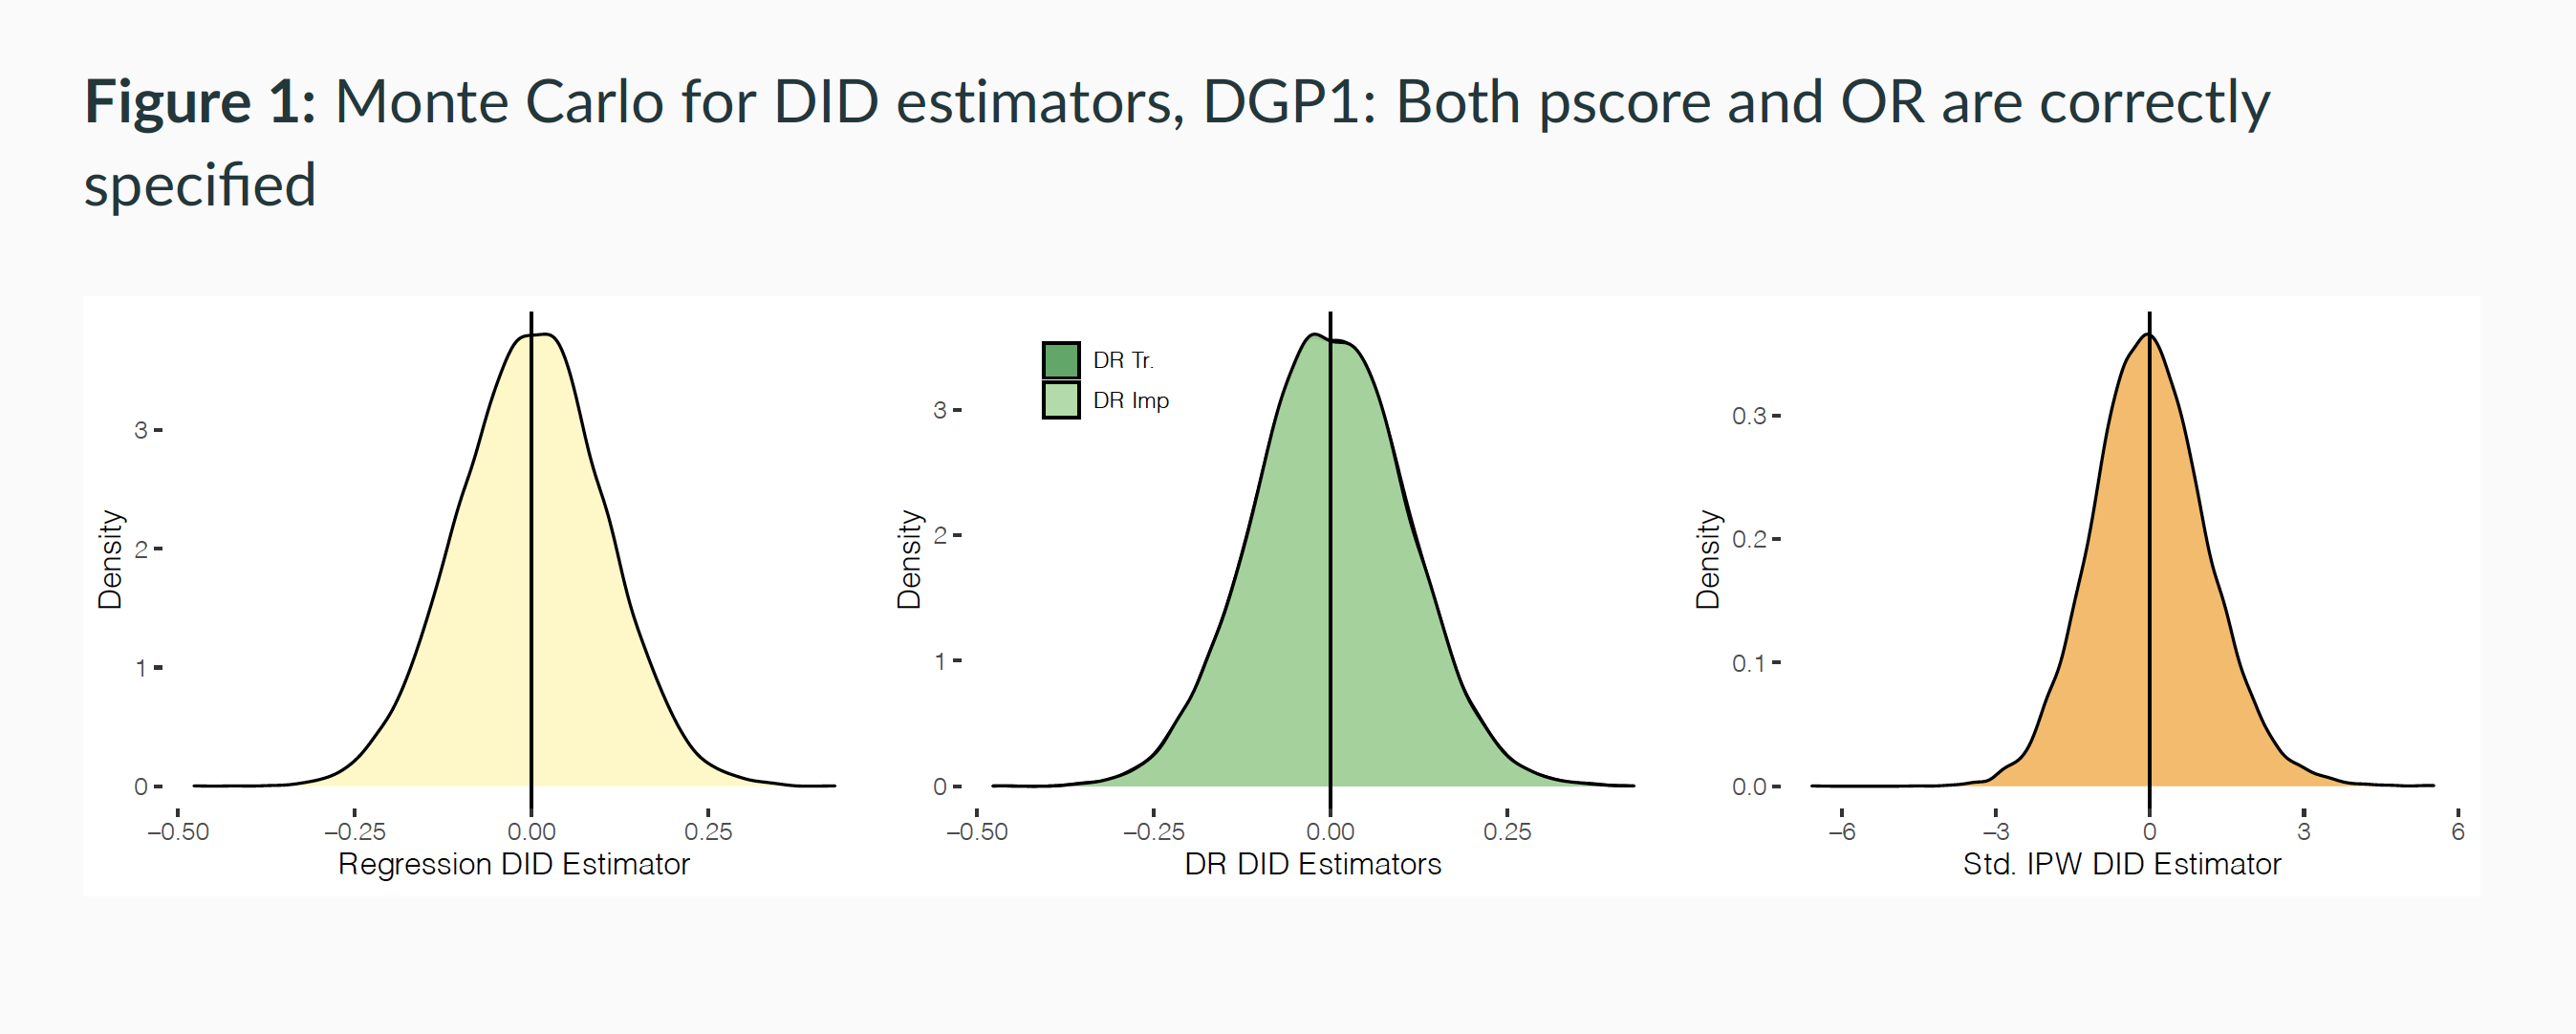
\includegraphics[scale=0.25]{./lecture_includes/mc_dr_1.png}
	\end{figure}

\end{frame}


\begin{frame}[plain]

\begin{table}[htbp]\centering
\scriptsize
\caption{Monte Carlo Simulations, DGP4, Neither OR and Propensity score correct}
\centering
\begin{threeparttable}
\begin{tabular}{l*{5}{c}}
\toprule
\multicolumn{1}{l}{\textbf{}}&
\multicolumn{1}{c}{\textbf{Bias}}&
\multicolumn{1}{c}{\textbf{RMSE}}&
\multicolumn{1}{c}{\textbf{SE}}&
\multicolumn{1}{c}{\textbf{Coverage}}&
\multicolumn{1}{c}{\textbf{CI length}}\\
\midrule
TWFE & -16.3846 & 16.5383 & 3.6268 & 0.000 & 14.2169 \\
OR & -5.2045 & 5.3641 & 1.2890 & 0.0145 & 5.0531 \\
IPW & -1.0846 & 2.6557 & 2.3746 & 0.9487 & 9.3084 \\
DR & -3.1878 & 3.4544 & 1.2946 & 0.3076 & 5.0749 \\
\bottomrule
\end{tabular}
\end{threeparttable}
\end{table}

\end{frame}

\begin{frame}[plain]
	\begin{figure}
	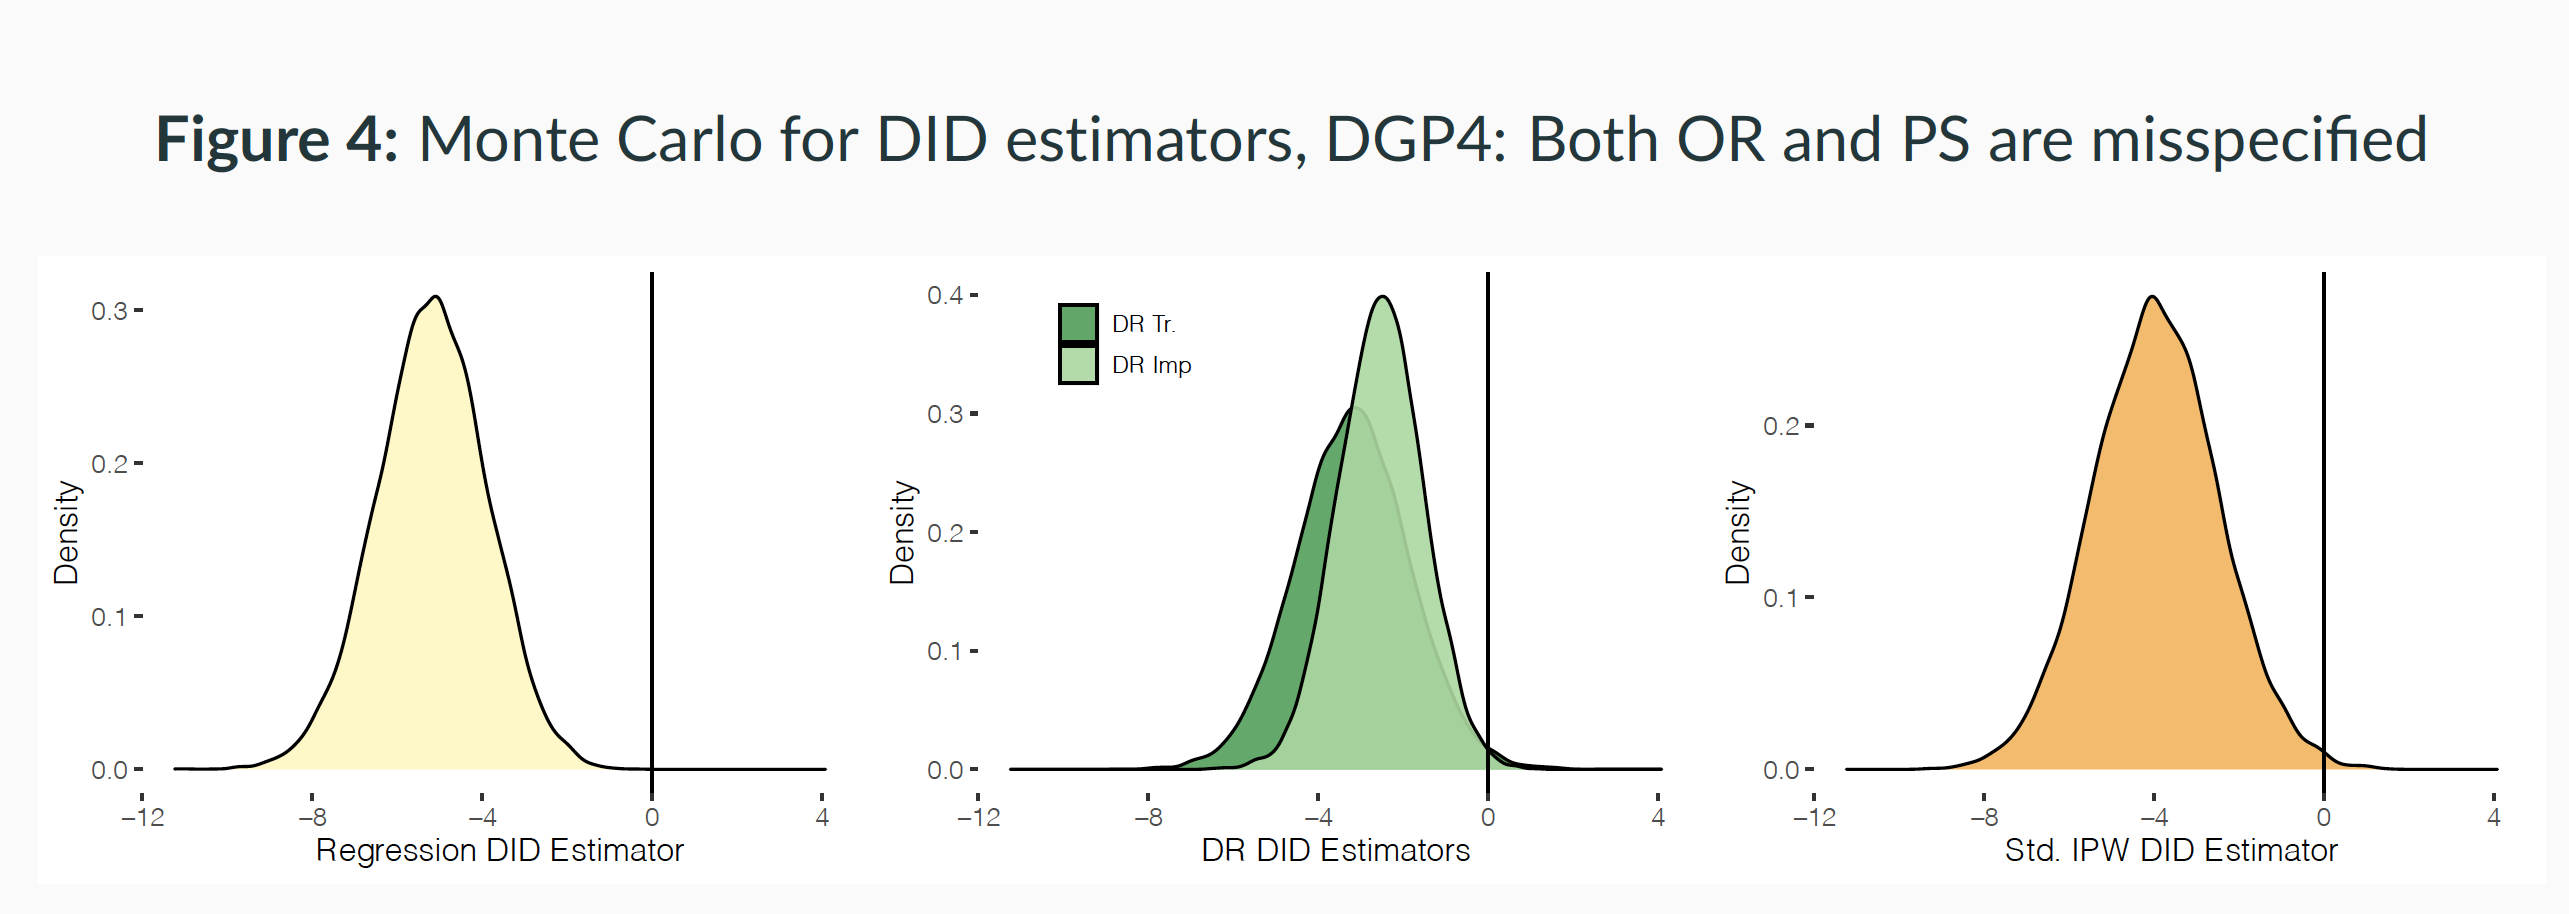
\includegraphics[scale=0.12]{./lecture_includes/mc_dr_2.png}
	\end{figure}


\end{frame}


\begin{frame}{Code}

There is code in R and Stata
\begin{itemize}
\item Stata: \textbf{drdid}
\item R: \textbf{drdid}
\end{itemize}
\bigskip
Remember -- it's for 2x2 with covariates (i.e., one treatment group)

\end{frame}




\begin{frame}{Concluding remarks}

\begin{itemize}
\item These two papers mark a different approach than is often the case for applied researchers who simply estimate regression models and hope they recover ``reasonably weighted'' causal effects
\item These new DiD start with target parameter and identification then build estimation
\item TWFE, as it turns out, is not mostly harmless
\end{itemize}

\end{frame}










\end{document}
